%% 使用 jnuthesis 文档类生成南京大学学位论文的示例文档
%%
%% 作者:胡海星,starfish (at) gmail (dot) com
%% 项目主页: http://haixing-hu.github.io/jnu-thesis/
%%
%% 本样例文档中用到了吕琦同学的博士论文的提高和部分内容,在此对他表示感谢.
%%

%% jnuthesis 文档类的可选参数有:
%%   nobackinfo 取消封二页导师签名信息.注意,按照南大的规定,是需要签名页的.
%%   phd/master/bachelor 选择博士/硕士/学士论文

% 使用 blindtext 宏包自动生成章节文字
% 这仅仅是用于生成样例文档,正式论文中一般用不到该宏包
\documentclass[bachelor,winfonts]{jnuthesis}

% 本科课程设计课程名称
\usepackage{graphicx}
\usepackage{subcaption}

\graphicspath{ {images/} }
%%%%%%%%%%%%%%%%%%%%%%%%%%%%%%%%%%%%%%%%%%%%%%%%%%%%%%%%%%%%%%%%%%%%%%%%%%%%%%%
% 设置论文的中文封面

% 如果论文标题过长,可以分两行,第一行用\titlea{}定义,第二行用\titleb{}定义,将上面的\title{}注释掉
\titlea{融合句子结构信息的文本理解}
\titleb{}

% 论文作者姓名
\author{胡勇}
% 论文作者学生证号
\studentnum{1030614418}
% 导师姓名职称
\supervisor{王澜}
\supervisorpos{讲师}
% 第二行导师姓名职称,仿照第一行填写,没有则留空
\supervisorb{}
\supervisorbpos{}
% 论文作者的学科与专业方向
\major{物联网工程}
% 论文作者所在院系的中文名称,学士学位论文此处不带“学院”二字
\department{物联网工程}
% 论文作者所在学校或机构的名称.此属性可选,默认值为``江南大学''.
\institute{江南大学}
% 学士学位获得日期,需设置年、月,默认为编译日期.
\bachelordegreeyear{2018}
\bachelordegreemonth{6}
%%%%%%%%%%%%%%%%%%%%%%%%%%%%%%%%%%%%%%%%%%%%%%%%%%%%%%%%%%%%%%%%%%%%%%%%%%%%%%%

%-------------------------------------------------------------------------------
%	CODE INCLUSION CONFIGURATION
%-------------------------------------------------------------------------------
\usepackage{listings}
\newfontfamily\menlo{Menlo}
\usepackage{color}
\lstset{
    columns=fixed,
    breaklines=true,
    numbers=left,                                        % 在左侧显示行号
    frame=single,                                        % 显示背景边框
    % backgroundcolor=\color[RGB]{245,245,244},            % 设定背景颜色
    % keywordstyle=\color[RGB]{40,40,255},                 % 设定关键字颜色
    numberstyle=\footnotesize\color{darkgray},           % 设定行号格式
    % commentstyle=\color[RGB]{0,96,96},                   % 设置代码注释的格式
    % stringstyle=\color[RGB]{128,0,0},                    % 设置字符串格式
    showstringspaces=false,                              % 不显示字符串中的空格
    basicstyle=\small\menlo,
    numberstyle=\scriptsize\menlo,
    xleftmargin=0cm,
    xrightmargin=0cm
}

\begin{document}

%%%%%%%%%%%%%%%%%%%%%%%%%%%%%%%%%%%%%%%%%%%%%%%%%%%%%%%%%%%%%%%%%%%%%%%%%%%%%%%

% 制作中文封面
\maketitle

%%%%%%%%%%%%%%%%%%%%%%%%%%%%%%%%%%%%%%%%%%%%%%%%%%%%%%%%%%%%%%%%%%%%%%%%%%%%%%%
% % 开始前言部分
% \frontmatter

%%%%%%%%%%%%%%%%%%%%%%%%%%%%%%%%%%%%%%%%%%%%%%%%%%%%%%%%%%%%%%%%%%%%%%%%%%%%%%%
% 论文的中文摘要
\begin{abstract}
自然语言理解(NLU)是自然语言处理乃至人工智能领域亟待解决的研究重点与难点.
近几年随着深度学习的发展,循环神经网络(RNN)因其强大的序列建模能力,在NLU任务取得了突破,有很好的结果.

% 中文关键词.关键词之间用中文全角分号隔开,末尾无标点符号.
\keywords{依存句法树;深度学习}
\end{abstract}

%%%%%%%%%%%%%%%%%%%%%%%%%%%%%%%%%%%%%%%%%%%%%%%%%%%%%%%%%%%%%%%%%%%%%%%%%%%%%%%
% 论文的英文摘要



\begin{englishabstract}
  In pattern recognition, the partition-based fuzzy clustering algorithm is one of the most commonly used algorithms in many clustering algorithms. In order to get a more systematic and in-depth understanding of these clustering algorithms and their properties, several fuzzy clustering algorithms are reviewed and evaluated. The advantages and disadvantages of these typical algorithms are compared and analyzed.

  Fuzzy C-Means (FCM) clustering is a simple, intuitive and easy-to-implement method for color image segmentation. In this paper, FCM is used to segment color images, and the clustering effectiveness is analyzed by Xie-Beni index to determine the number of clusters. Experiments show that FCM clustering algorithm can cluster the color of the image to achieve color image segmentation.
% 英文关键词.关键词之间用英文半角逗号隔开,末尾无符号.
\englishkeywords{Fuzzy Clustering, C-means, Color Image Segmentation}
\end{englishabstract}

%%%%%%%%%%%%%%%%%%%%%%%%%%%%%%%%%%%%%%%%%%%%%%%%%%%%%%%%%%%%%%%%%%%%%%%%%%%%%%%
% 生成论文目次
\tableofcontents

%%%%%%%%%%%%%%%%%%%%%%%%%%%%%%%%%%%%%%%%%%%%%%%%%%%%%%%%%%%%%%%%%%%%%%%%%%%%%%%
% 开始正文部分
\mainmatter

%%%%%%%%%%%%%%%%%%%%%%%%%%%%%%%%%%%%%%%%%%%%%%%%%%%%%%%%%%%%%%%%%%%%%%%%%%%%%%%
% 学位论文的正文应以《绪论》作为第一章

%第一章绪论
\chapter{绪论}\label{chapter_introduction}
\section{研究背景和意义}
自然语言处理(Natural Language Processing,NLP)是研究计算机处理人类语言的一门技术,也是人工智能(Artificial Intelligence,AI)最初发展的切入点和当前关注的焦点.

人工智能体系可分为运算智能、感知智能、认知智能三个层次(图1-1).其中,最后的认知智能的发展主要体现为自然语言处理技术的进步.
如果语言智能够实现突破,与它同属认知智能的知识和推理就会得到长足的发展,进而推动整个人工智能体系进步,让更多的应用场景落地.
所以自然语言处理技术也被认为是人工智能皇冠上的明珠.

而自然语言理解(Natural Language Understanding,NLU)技术则是对语义信息的深层次挖掘和处理,是NLP技术当前研究的重点和难点.
广义的自然语言理解可以分为两类,第一类是针对口语内容的理解,如语音识别,语音解析和语音合成;
第二类是对书面文本的理解,也是本文主要讨论的内容,即本文题中的文本理解(Text understanding).
人工智能,自然语言处理,自然语言理解和文本理解的关系可以表示为下图.

\begin{figure}[h!]
  \centering
  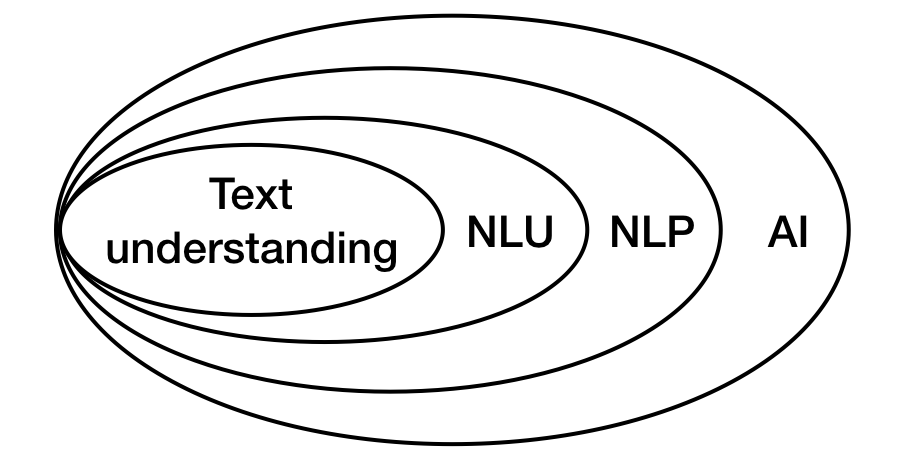
\includegraphics[width=0.5\linewidth]{结构关系.png}
  \caption{人工智能,自然语言处理,自然语言理解和文本理解的关系}
\end{figure}

文本理解技术是众多高级NLP应用不合或缺的一项核心技术,这些应用包括文本分类、信息抽取、自动摘要、机器翻译、问答系统等.

(1)文本分类:文本分类是文本处理中的一个重要模块,它的应用也非常广泛,比如:垃圾过滤、新闻分类、词性标注等.
它和其他的分类没有本质的区别,核心方法为首先提取分类数据的特征,然后选择最优的匹配,从而分类.

(2)信息抽取:信息抽取 是把文本里包含的信息进行结构化处理,变成表格一样的组织形式.
输入信息抽取系统的是原始文本,输出的是固定格式的信息点.
信息点从各种各样的文档中被抽取出来,然后以统一的形式集成在一起.

(3)自动摘要:随着近几年文本信息的爆发式增长,人们每天能接触到海量的文本信息,如新闻、博客、聊天、报告、论文、微博等.
从大量文本信息中提取重要的内容,已成为我们的一个迫切需求,而自动文本摘要就提供了一个高效的解决方案,
可以从原文本中提炼出简洁而重要的信息.

(4)机器翻译:机器翻译,又称为自动翻译,是利用计算机将一种自然语言(源语言)转换为另一种自然语言(目标语言)的过程.
它是计算语言学的一个分支,是人工智能的终极目标之一,具有重要的科学研究价值.
同时,机器翻译又具有重要的实用价值.随着经济全球化及互联网的飞速发展,机器翻译技术在促进政治、经济、文化交流等方面起到越来越重要的作用.

(5)问答系统:问答系统是信息检索系统的一种高级形式,它能用准确、简洁的自然语言回答用户用自然语言提出的问题.
这种交互一直认为是最自然的人机交互方式,随着苹果Siri,微软Cortana,天猫智能客服的推出,智能问答系统成为备受关注的热点研究方向.

(6)舆情分析:舆情是指社会空间中群众对社会事件发生,发展,变化持有的态度、意见、情绪等表现的总和.
网络中的舆情主要来源包括微博,BBS论坛,新闻评论等.显然舆情分析是一项复杂的综合性技术,涉及到网络文本内容挖掘,
观点意见挖掘等.

\begin{figure}[h!]
  \centering
  \begin{subfigure}[b]{0.4\linewidth}
    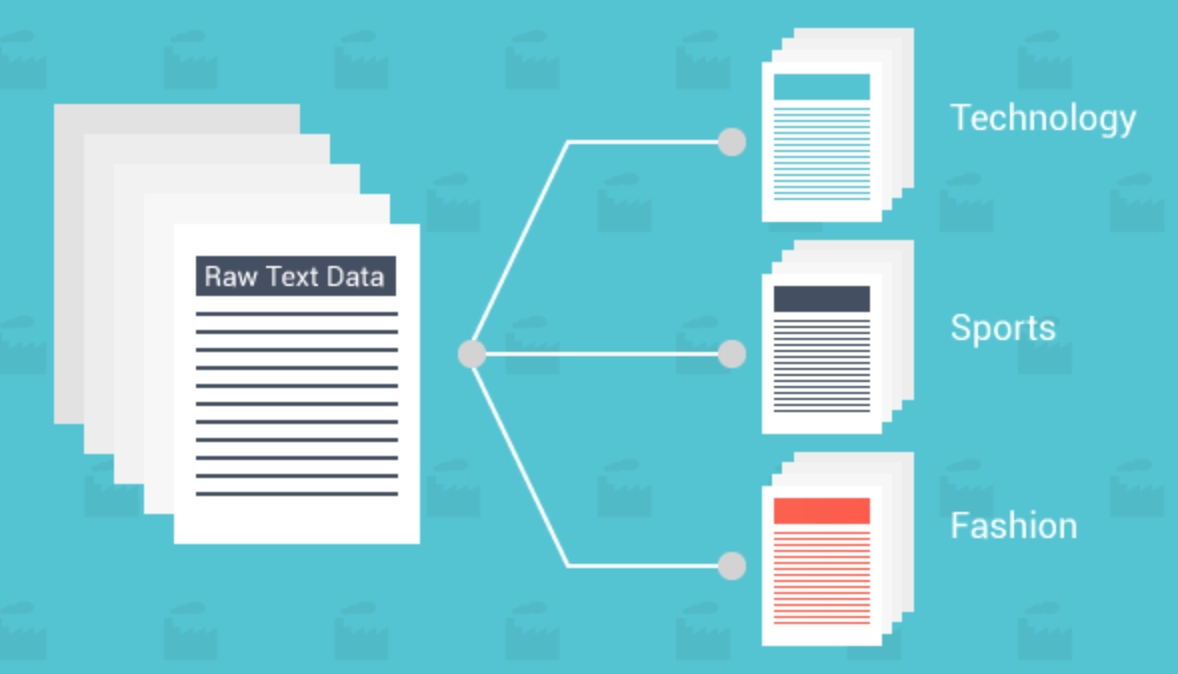
\includegraphics[width=\linewidth]{文本分类.png}
    \caption{文本分类}
  \end{subfigure}
  \begin{subfigure}[b]{0.4\linewidth}
    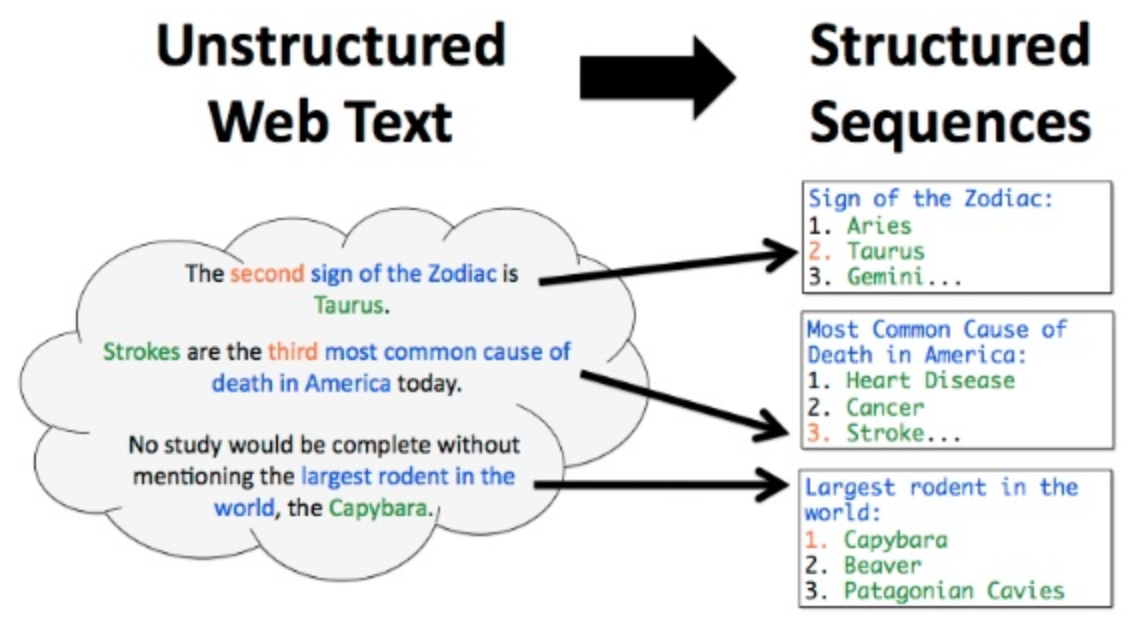
\includegraphics[width=\linewidth]{信息抽取.png}
    \caption{信息抽取}
  \end{subfigure}
  \begin{subfigure}[b]{0.4\linewidth}
    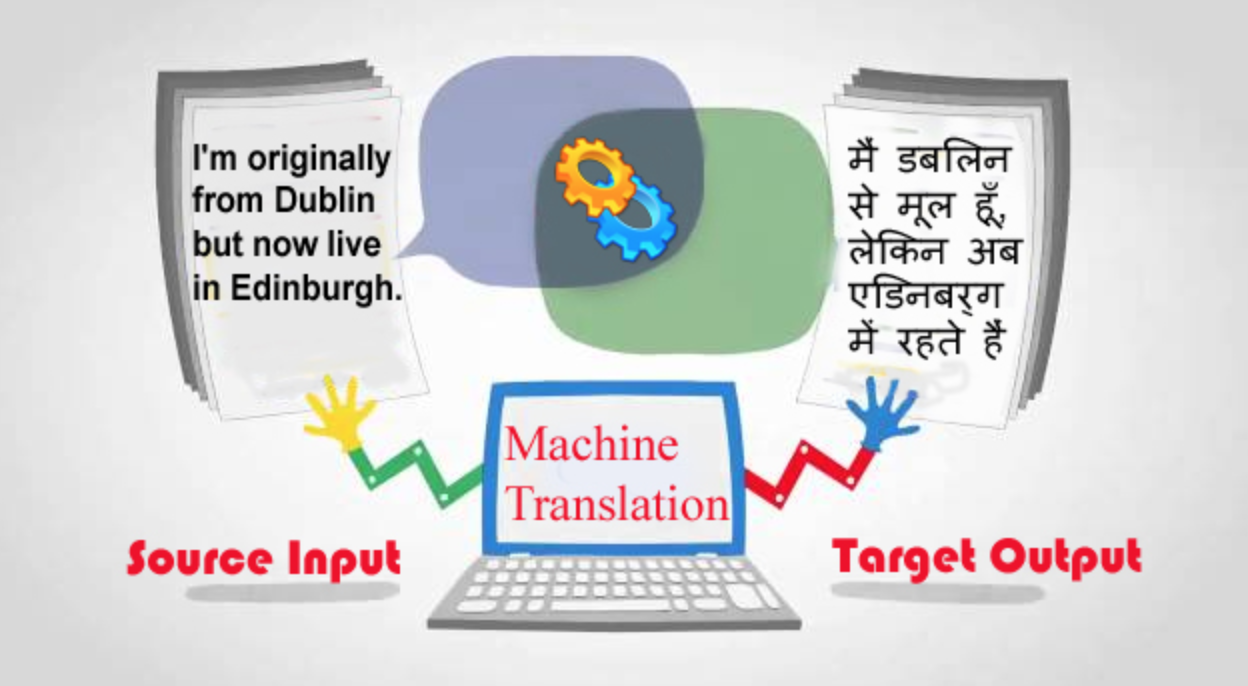
\includegraphics[width=\linewidth]{机器翻译.png}
      \caption{机器翻译}
  \end{subfigure}
  \begin{subfigure}[b]{0.4\linewidth}
    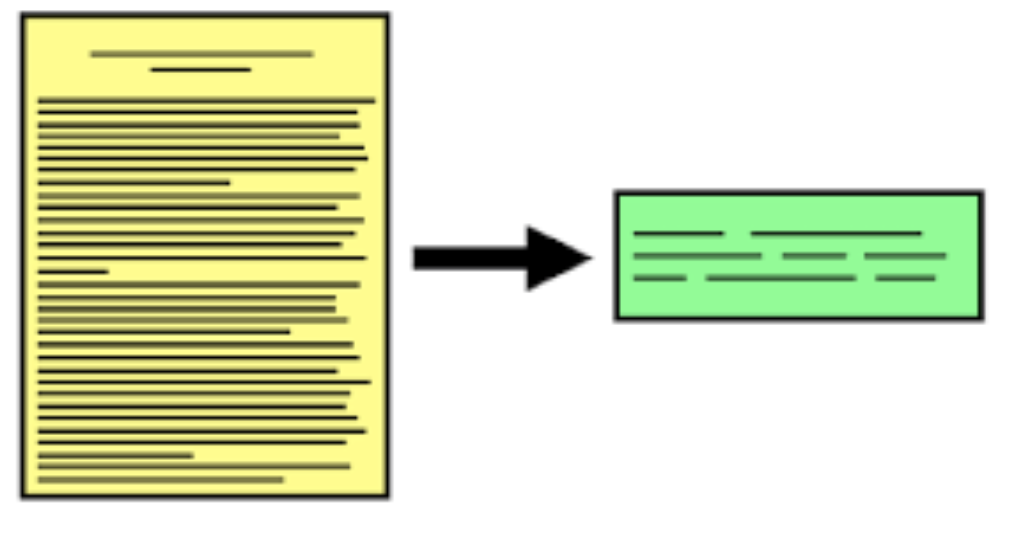
\includegraphics[width=\linewidth]{自动摘要.png}
    \caption{自动摘要}
  \end{subfigure}
  \begin{subfigure}[b]{0.4\linewidth}
    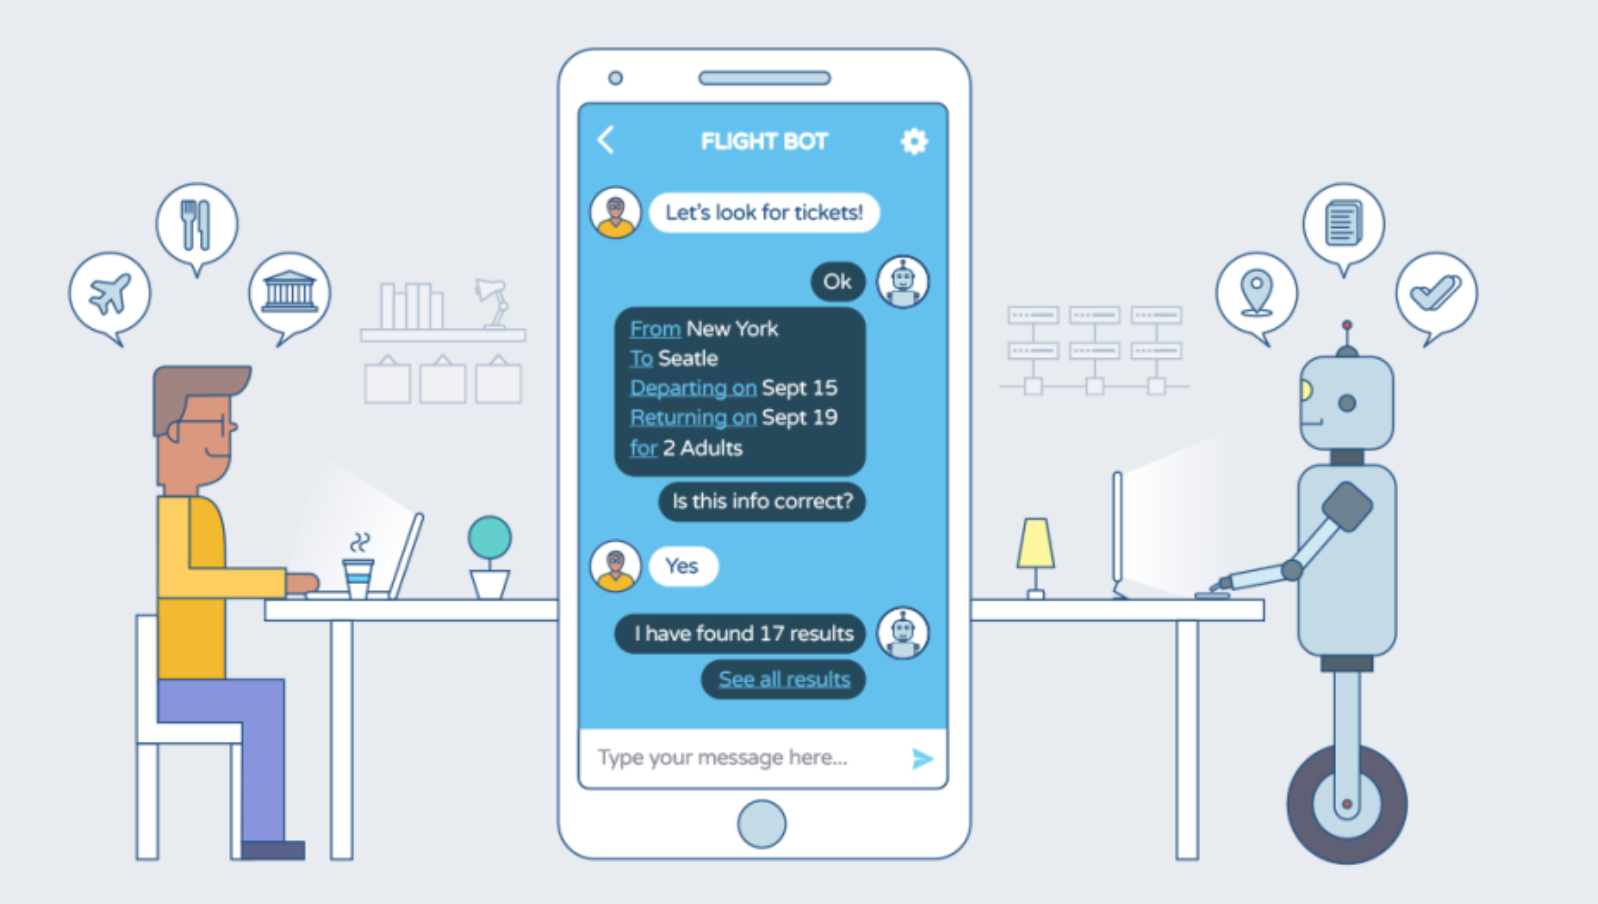
\includegraphics[width=\linewidth]{问答系统.png}
    \caption{问答系统}
  \end{subfigure}
  \begin{subfigure}[b]{0.4\linewidth}
      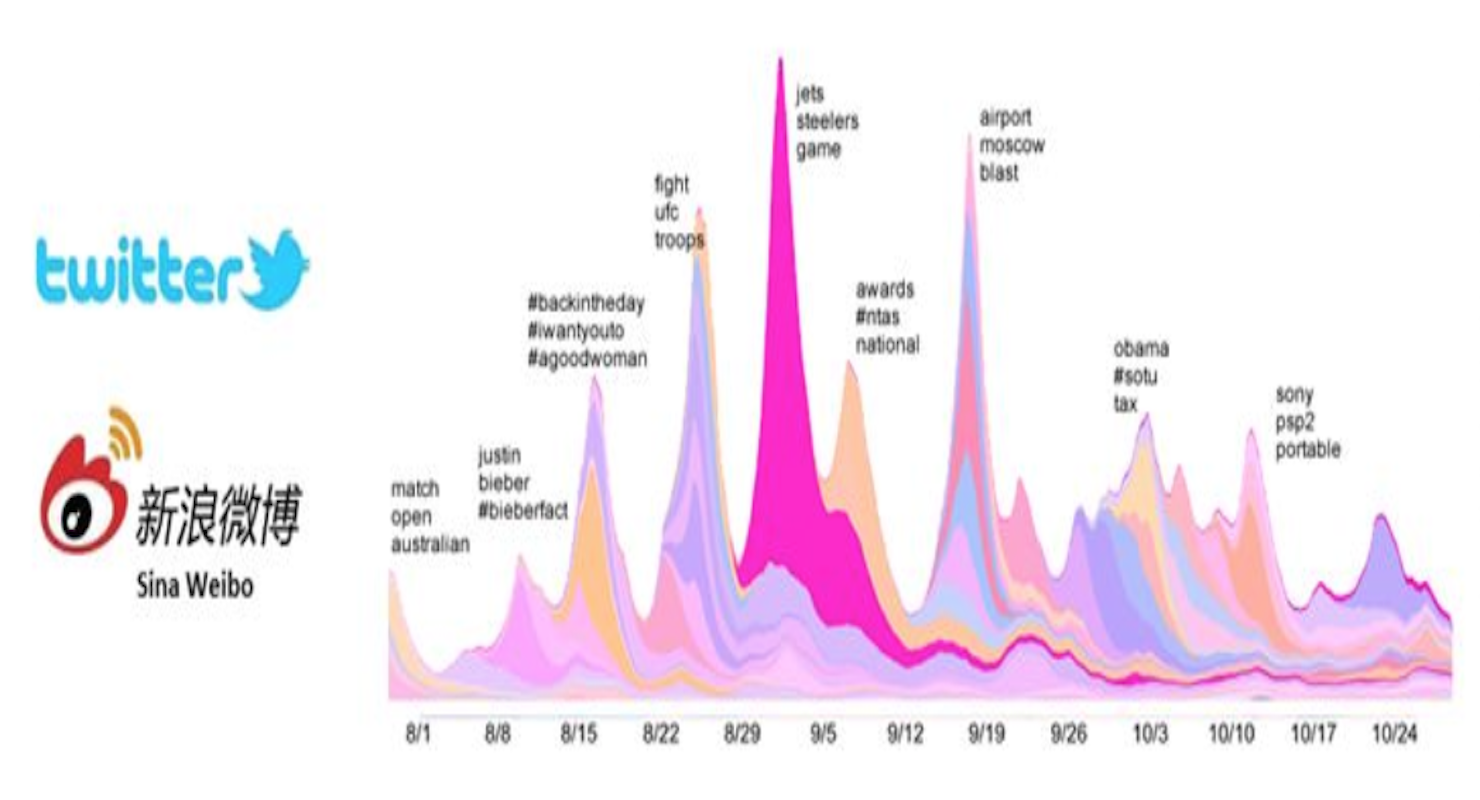
\includegraphics[width=\linewidth]{舆情分析.png}
      \caption{舆情分析}
  \end{subfigure}
  \caption{文本理解的相关应用}
\end{figure}


所以对文本理解技术的研究必然可以推动NLP领域的发展,从而直接或间接推动这些应用的性能和实用性的提高,具有重要的研究意义和价值.

\section{文本理解研究的发展与现状}
\subsection{文本理解的早期发展}
文本内容理解的研究最早是从1954年的Georgetown大学的机器翻译系统研发开始的,
但是一开始是通过制定规则的语法入手,所以在系统构建上有很大的局限性,带来了翻译质量的低劣.
随着研究的深入,基于规则的思路面临越来越多的困难.1966年,美国科学院语言自动处理委员会(Automatic Language Processing Advisory Committee)
公布了一个题为《语言与机器》的报告(简称ALPAC报告),该报告全面否定了机器翻译的可行性,并建议停止对机器翻译项目的资金支持.

此后一段时间对与机器翻译的研究跌倒了谷底,但是研究者仍然坚持对计算语言的理论进行研究,并产生了很多非常重要的研究成果,
比如在句法研究上1969年J.Earley提出的Earley句法分析算法等,在语义分析上1966年C.J.Filmore提出的格语法等.

直到80年代后期,人们通过构建语料库,把基于语料库的统计方法引入到自然语言处理中,
尤其是把已经在语音识别中取得成功的隐马尔可夫模型(Hidden Markov Model,HMM)引入到自然语言处理上,
起到了推波助澜的效果,很多人开始通过在大规模语料库上运用统计机器学习方法,并量化的评价和比较各种评价方法的性能.

此后自然语言处理领域的研究从基于规则方法转到基于统计的方法.

\subsection{文本理解的研究现状}
Ruhi Sarikaya在2011年指出一个自然语言理解系统包括3个任务:
领域识别(domain detection),意图分类(intent determination)和属性抽取(slot filling)\cite{Deepbelief},
它们是一个连续的过程,首先识别文本领域,之后对用户意图进行分类,最后实现属性抽取.

从技术上讲,领域识别和意图分类是一个分类问题,通常使用传统的分类算法实现,
如2003年Haffner等人提出的支持向量机(Support Vector Machine,SVM)\cite{SVM}和
Chelba等人提出的最大熵算法(Maximum Entropy Classifier).
2014年Chen等人提出也可以采用神经网络(Neural Network Classifier)来解决该问题.
而对于属性抽取则可以认为是一个序列标注问题,可以运用隐马尔可夫模型
和条件随机场(Conditional Random Field,CRF) 模型解决.

随着深度学习的发展,神经网络模型也被应用来处理领域识别和意图分类问题.
值得注意的是,Recently, Ravuri 和Stolcke 在2015年提出可采用循环神经网络(Recurrent Neural Network,RNN)来解决意图分类问题.
而对于属性抽取,可通过深度学习来提取特征并与传统的CRF相结合.Mesnil也尝试使用RNN进行序列标注以实现属性抽取.

循环神经网络经过实验证明在对序列化建模上效果显著,能够利用和记忆上下文信息,在几乎所有的NLP任务上都有很好的表现.
但是循环神经网络在反向传播求解的过程中会出现梯度消失和梯度爆炸的问题,所以对于长文本建模效果不佳.
后期提出的长短期记忆网络(Long Short-Term Memory,LSTM),通过在隐藏层设置3个“门”的结构,选择性的记忆和忘记,有效的解决了长文本建模的问题.
后来在此基础上有演化出许多改进的模型,比如树结构的长短期记忆网络(Tree-LSTM),双向的长短期记忆网络(Bi-LSTM),
用来解决不同场景下的序列建模,如文本分类,中文分词,语义解析等.

目前以RNN为代表的深度学习模型已经成为了自然语言理解研究的主流方法.

但是上述研究均需要大量训练数据,并且一切都处于深度神经网络的黑盒中,使整个模型缺乏必要的直观性和鲁棒性.
而且最重要的是这种模型忽略了句子中的结构信息及语言学知识,而这些知识是可以用来辅助提升模型的,比如对于训练语料库中未出现的句子的词序列标注.

因此将语言的先验知识融入深度学习可以提高框架的可解释性和鲁棒性,将是 NLP 未来发展的重要方向.



\section{论文主要工作和贡献}
本文围绕研究将语言中的先验知识与深度学习模型进行有机融合,提出了融合依存句法结构的深度神经网络,并基于文本分类任务,研究融合模型的效果.
具体来说,本文的研究内容可以归纳为以下几个方面.

(1)通过斯坦福句法分析工具,构建文本的依存句法树,解析出子文本结构.

(2)研究和复现传统的RNN、LSTM等深度神经网络模型,并在LSTM模型的基础上融合依存句法信息.

(3)研究和比较子文本结构的Attention对网络性能的影响,包括concatention-based、dot、bi-liner Attention.

(4)研究和比较多种融合方式对网络性能的影响,包括简单的加和融合、带权重系数的加权融合、特征串联融合等.


\section{论文结构安排}
本论文总共分为五个部分,各章节具体安排如下:

(1)第一章为绪论,该章首先介绍了文本理解的研究背景及意义,然后介绍了该领域的研究发展和 现状,并且简单描述了本文的研究内容,最后给出了全文的结构安排.

(2)第二章为基于深度学习的文本理解,包括Word Embedding的文本表示方法,RNN、LSTM深度学习模型的介绍以及给予深度学习的依存句法分析.

(3)第三章为融合句法结构树的深度神经网络模型,详细介绍了融合模型的设计步骤和方案.

(4)第四章为实验部分,基于语料库AG-News,设计了RNN,LSTM和融合句法结构树的深度神经网络在分类任务上的对照实验,
并且对融合网络中的Attenion方式,融合方式分别进行了对照实验.
实验证明了本文提出的模型在文本理解上的有效性和可行性.

(5)第五章为结论与展望,该章对本文的主要工作进行了总结,并对下面的工作进行了展望.

\chapter{基于深度学习的文本理解}
\section{文本的词向量表示方法}
自然语言处理领域最小的单元就是词语,通过词语构成句子,再有句子构成篇章.
所以为了让计算机能够处理文本首要任务就是对词语进行表示.
好的文本表示能够更加真是的反应文本的内容,对于不同的内容有更好的区分能力.

现在主流的表示方法是基于词向量(word embedding)的文本表示.
通过词向量可以讲词转化成稠密向量,对于相似的词,对应的词向量也相近.
这种表示方法又可以分为独热表示(one-hot representation)和分布式表示(distributed representation).

\subsection{独热表示}
用词向量表示文本,独热表示是一种最直接也是最简单的表示方法.
具体来说,每个词都表示成一个$n$维的向量,这里$n$为语料库中词表的大小.
假设某个单词在词表中的位置是$k$,那么这个单词的词向量只有位置$k$是1,
其他位置均是0.

比如有一个句子“我喜欢音乐,尤其是摇滚和嘻哈.”
如果整个语料库中就仅有这一个句子,这个句子分词后有8个不重复的单词,所以每个单词都可以表示为一个8维的向量,如下表所示.

\begin{table}[h!]
  \centering
  \begin{tabular}{cccccccc}
    \toprule
    \textbf{我} & \textbf{喜欢} & \textbf{音乐} & \textbf{尤其} & \textbf{是} & \textbf{摇滚}  & \textbf{和} & \textbf{嘻哈}  \\
    \midrule
    1 & 0 & 0 & 0 & 0 & 0 & 0 & 0 \\
    0 & 1 & 0 & 0 & 0 & 0 & 0 & 0 \\
    0 & 0 & 1 & 0 & 0 & 0 & 0 & 0 \\
    0 & 0 & 0 & 1 & 0 & 0 & 0 & 0 \\
    0 & 0 & 0 & 0 & 1 & 0 & 0 & 0 \\
    0 & 0 & 0 & 0 & 0 & 1 & 0 & 0 \\
    0 & 0 & 0 & 0 & 0 & 0 & 1 & 0 \\
    0 & 0 & 0 & 0 & 0 & 0 & 0 & 1 \\
    \bottomrule
  \end{tabular}
  \caption{8维独热词向量表示}\label{table:3t1}
\end{table}

这种表示方案如果采用稀疏方式存储,会是非常的简洁:也就是给每个词分配一个数字ID.
比如刚才的例子中,音乐记为2,摇滚记为5(从0开始记),如果要编程实现的话,用Hash表给每个词分配一个编号即可.
这么简洁的表示方法配合上最大熵、SVM、CRF等算法已经很好地完成了NLP领域的各种主流任务了.

但是这种表示方法也存在一个重要的问题就是“词汇鸿沟”现象:任意两个词之间都是孤立的,词向量之间都是正交.
光从两个向量中看不出两个词是否有关系,比如例子中的音乐和摇滚在语义上是相关的,但这种相关性无法从词向量上体现出来.

\subsection{分布式表示}
为了解决独热法无法体现语义的问题,Hinton在1986年提出了一种新的表示方法:Distributed representation,也就是“分布式表示”.
基本思想是通过训练将每个词映射成 K 维实数向量(K一般为模型中的超参数),通过词之间的距离(比如 cosine 相似度、欧氏距离等)来判断它们之间的语义相似度.

2003年Bengio提出了一种经典的三层的神经网络“输入层-隐层-输出层”模型来训练词向量.
其核心思想是:一个给定单词的意思是由它的上下文确定的.
通过将被预测词的前$n$个词连接后作为神经网络的输入项,最后通过softmax层计算得到改词的词向量表示.
这种训练得到的词向量有很强的语义相关,
例如,$V(\mbox{意大利})-V(\mbox{罗马})+V(\mbox{巴黎}) = V(\mbox{法国})$,
类似的,$V(\mbox{国王})-V(\mbox{男人})+V(\mbox{女人})=V(\mbox{女王})$.
这样的结果非常振奋人心,但是这个算法对计算要求很高,训练效率较低.

2013年Google的Mikolov提出了Word2vec工具包,里面包括了两种新的词向量模型:
CBOW(continuous bag of words)模型:给定上下文次,预测是否是中心词
和skip-gram模型:给定中间词,预测是否是上下文词.
工具包中还包括了两种高效训练的方法:负采样(negative sampling)和层序softmax(hierarchical softmax).
Word2vec大受欢迎的原因正是其高效性,Mikolov在论文中指出,一个优化的单机版本一天可训练上千亿词.

\begin{figure}[h!]
  \centering
  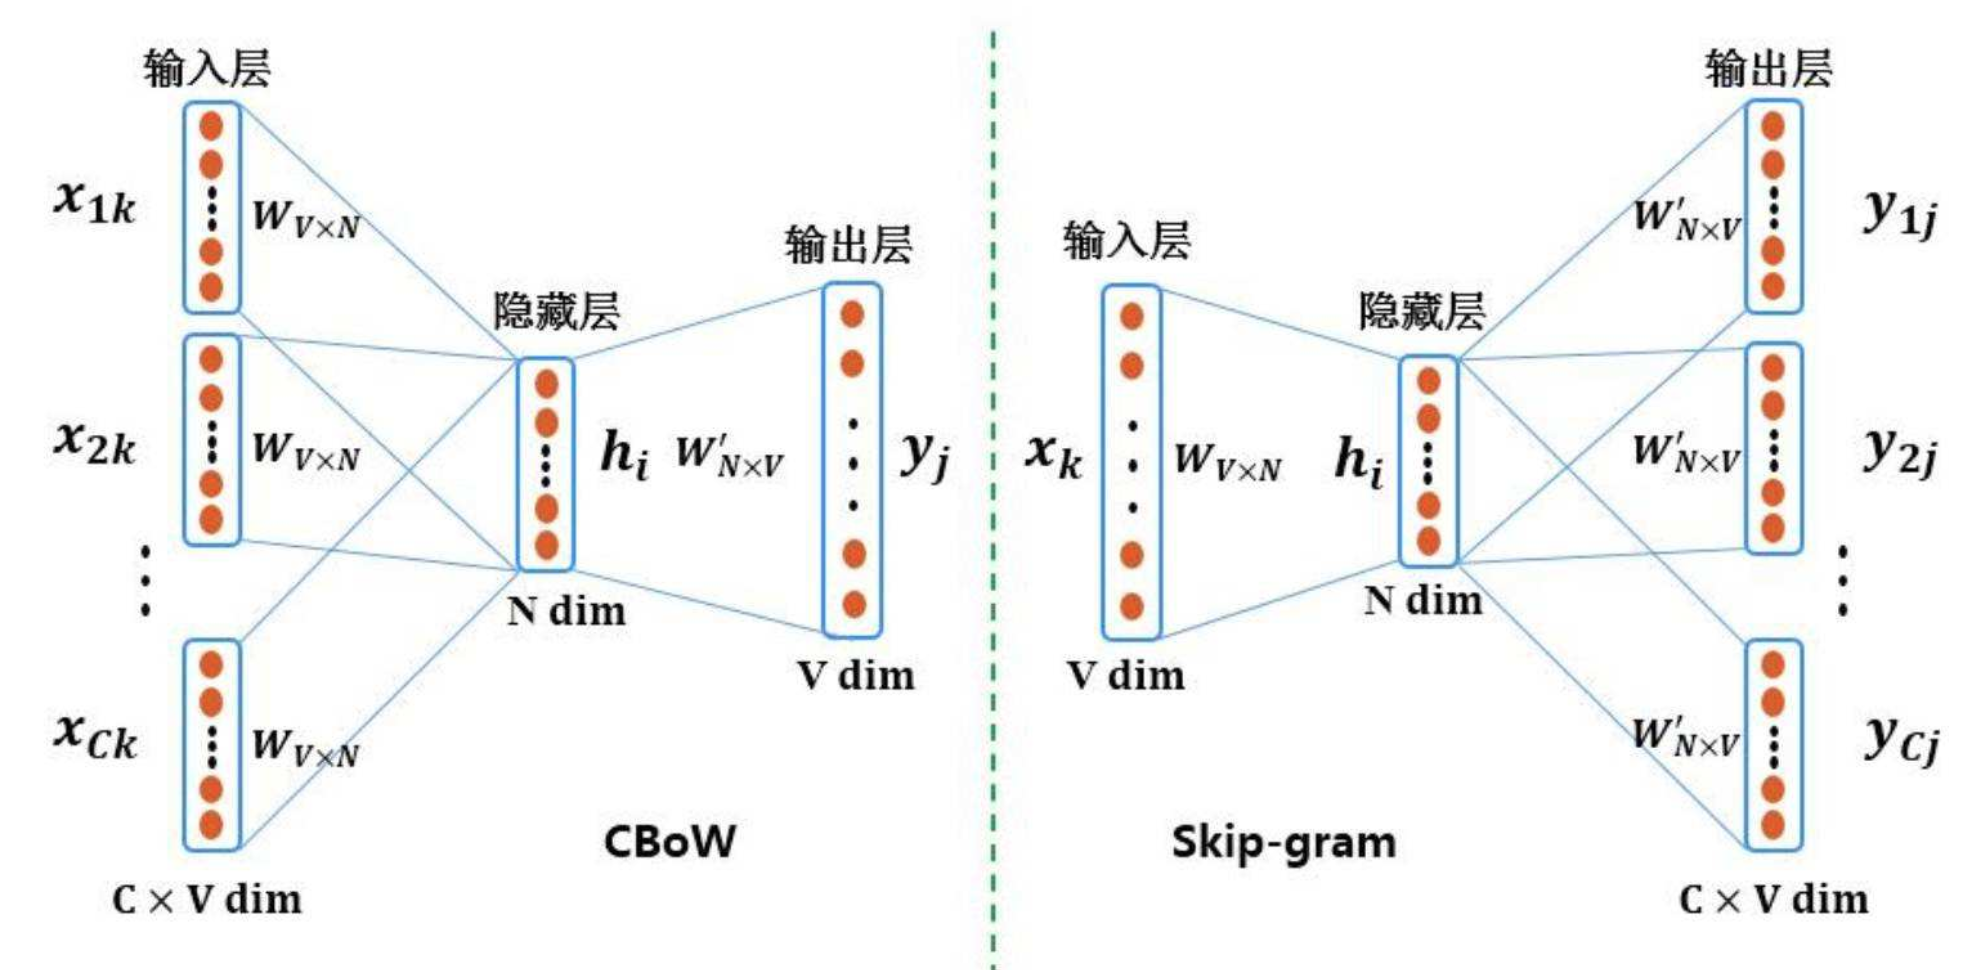
\includegraphics[width=0.6\linewidth]{CBOW-skip-gram.png}
  \caption{CBOW和skip-grams模型图示}
\end{figure}

具体来说,遍历文本中的每一个位置,包括一个中心词$c$和上下文单词$o$,通过词向量的$c$与$o$的相似度来计算$o$是$c$上下文的可能性,
通过调整词向量使得全局可能性达到最大.对于每个位置$t$,中心单词为$w_{t}$,窗口大小为$m$,那么全局可能性为:

\begin{equation}
  L(\theta) = \prod_{t=1}^{T} \prod_{-m \le j \le m ;j \neq m} P(w_{t+j}|w_{t},\theta)
\end{equation}

所以损失函数可以写成:
\begin{equation}
  J(\theta) = -\frac{1}{T}logL(\theta) = -\frac{1}{T} \sum_{t=1}^{T} \sum_{-m \le j \le m ;j \neq m} log P(w_{t+j}|w_{t},\theta)
\end{equation}

其中概率$P$通过$softmax$函数计算,采用梯度下降算法训练参数.

\subsection{GloVe模型}
Word2vec是基于局部上下文进行词向量训练的,所以并没有考虑到全局的信息.
2014年斯坦福大学的Jeffrey Penninngton等人提出了无监督学习的Glove(Global Vectors for Word Representation)模型.

其主要思想是以某个词的上下文窗口遍历整个语料库,统计窗口中词与词共同出现的次数,得倒整个语料库的词共现矩阵,
最后利用矩阵中的非零元素训练词向量.

设整个词共现矩阵为$X$,那么$X_{i}$为单词$w_{i}$上下文中所有出现词的总和,也就是矩阵第$i$行的和
,$X_{i,j}$表示单词$w_{i}$上下文中$w_{j}$出现的次数.那么单词$w_{j}$在$w_{i}$上下文中的概率为:

\begin{equation}
  P_{i,j} = P(w_{j}|w_{i}) = \frac{X_{i,j}}{X_{i}}
\end{equation}

两个词的共现概率就可以体现两个词的相关性.给定一个词$w_{k}$,通过计算$p_{ki}$ 与$p_{kj}$的比值,
来判断$w_{i}$和$w_{j}$哪一个与$w_{k}$更相关,如果比值大于1,则是单词$w_{i}$,反之就是单词$w_{j}$.
模型中词与词之间共现概率的比值可以最终转换成需要优化的目标函数:

\begin{equation}
  J = \sum_{i,j}^{N}f(X_{i,j})(v_{i}^{T}v_{j}+b_{i}+b_{j}-log(X_{i,j}))^2
\end{equation}

其中$v_{i}$,$v_{j}$是单词$i$和单词$j$的词向量,
$b_{i}$,$b_{j}$是两个标量,作者定义的偏差项,
$N$是词汇表的大小,共现矩阵维度为$N*N$,$f$是权重函数,需要满足一定的非递减性,
来保证对低频词共现组合不会赋值很大,所以一般$f(X_{i,j})$定义为:

\begin{equation}
  f(x) = 
  \left\{
    \begin{array}{lr}
      (x/x_{max})^{\alpha}, & x<x_{max} \\
      1, & x \ge x_{max} 
    \end{array}
    \right.
\end{equation}

其中,$\alpha$一般取$0.75$,$x_{max}$则根据语料库的实际情况而定.


\section{NLP领域的深度学习模型}
神经网络模型具备强大的学习能力和拟合能力,在图像,音频,NLP等诸多领域取得了非常好的效果.
NLP领域应用最为广泛的深度学习模型就是循环神经网络RNN和长短期记忆网络LSTM.

\subsection{循环神经网络}
传统的神经网络并不能做到持续记忆,这也应该是传统神经网络的一个缺陷.
如果让神经网络对电影中每个时间点的事件进行分类,很明显,传统神经网络不能使用前一个事件去推理下一个事件.
循环神经网络RNN的出现很好的解决了对序列数据建模的问题.

RNN之所以称为循环神经网路,是因为一个序列当前的输出与前面的输出有关.
具体的表现形式为网络会对前面的信息进行记忆并应用于当前输出的计算中,
即隐藏层之间的节点不再无连接而是有连接的,
也就是说隐藏层的输入不仅包括输入层的输出还包括上一时刻隐藏层的输出.
下图是一个典型的RNN结构图:

\begin{figure}[h!]
  \centering
  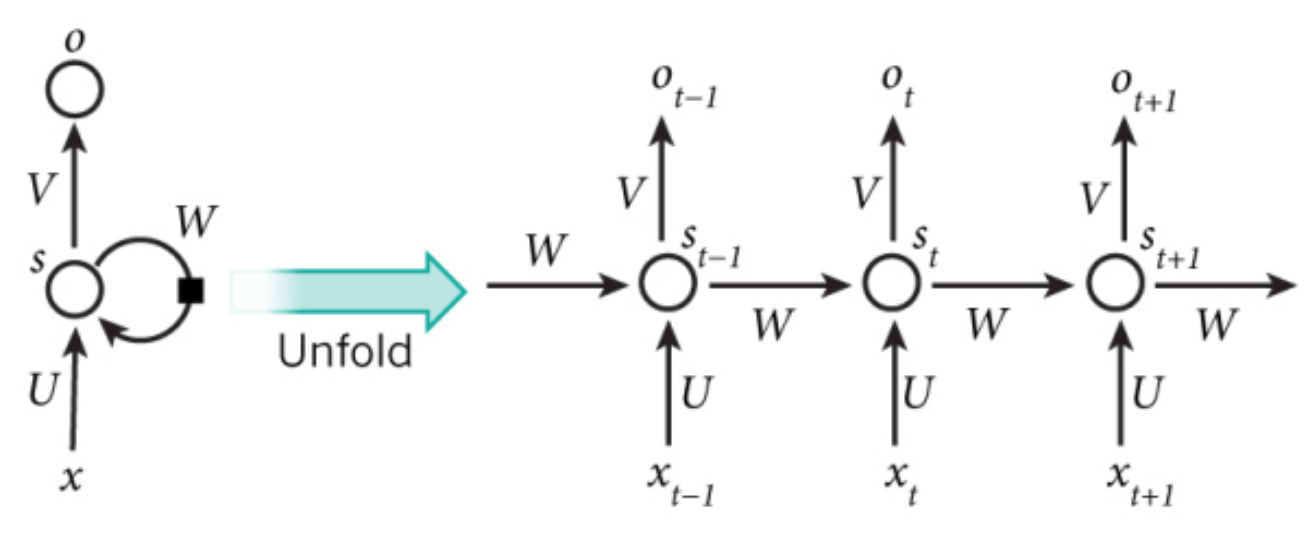
\includegraphics[width=0.6\linewidth]{RNN.png}
  \caption{RNN结构图}
\end{figure}

如图所示,把循环神经网络进行展开成一个全神经网络.
例如,对一个包含3个单词的语句,那么展开的网络便是一个有3层神经网络,每一层代表一个单词.
其中$x_{t}$表示第$t$步的输入,$s_{t}$为隐藏层的第$t$步的状态,它是网络的记忆单元.
$s_{t}$根据当前输入层的输出与上一步隐藏层的状态进行计算,$o_{t}$是第t步的输出.

\begin{equation}
  \left\{
  \begin{array}{l}
    s_{t} = f(U*x_{t}+W*s_{t-1}) \\
    o_{t} = softmax(V*s_{t})
  \end{array}
  \right.
\end{equation}

上式中的$f$表示非线性的激活函数,如$tanh$,$ReLU$.
需要注意的是:在RNN中,每输入一步,每一层各自都共享参数$U$,$V$,$W$.
其反映着RNN中的每一步都在做相同的事,只是输入不同,
因此大大地降低了网络中需要学习的参数.



\subsection{长短期记忆网络}


\section{依存句法分析}

\chapter{结语}


% 参考文献.应放在\backmatter之前.
% 推荐使用BibTeX,若不使用BibTeX时注释掉下面一句.
\nocite{*}
\bibliography{bachelor}
% 不使用 BibTeX
%\begin{thebibliography}{2}
%
%\bibitem{deng:01a}
%{邓建松,彭冉冉,陈长松}.
%\newblock {\em \LaTeXe{}科技排版指南}.
%\newblock 科学出版社,书号:7-03-009239-2/TP.1516, 北京, 2001.
%
%\bibitem{wang:00a}
%王磊.
%\newblock {\em \LaTeXe{}插图指南}.
%\newblock 2000.
%\end{thebibliography}

%%%%%%%%%%%%%%%%%%%%%%%%%%%%%%%%%%%%%%%%%%%%%%%%%%%%%%%%%%%%%%%%%%%%%%%%%%%%%%%
% 致谢,应放在《结论》之后
\begin{acknowledgement}
  本文是在模式识别葛洪伟老师的悉心指导下完成的,非常感谢葛洪伟老师.

  感谢江南大学物联网工程学院给我提供了一个学习的平台.

  感谢《机器学习实战》的作者以及《模式识别与智能计算》的作者.这两本书对我的学习有很大的帮助.

  感谢胡海星、王雪瑞学长提供\LaTeX 模板.

  感谢我的父母,对我在学习上的支持和鼓励.
  
\end{acknowledgement}

\backmatter




%%%%%%%%%%%%%%%%%%%%%%%%%%%%%%%%%%%%%%%%%%%%%%%%%%%%%%%%%%%%%%%%%%%%%%%%%%%%%%%
\end{document}
